\RequirePackage{luatex85}
\documentclass[tikz]{standalone}
% Default preamble
\usepackage{pgfplots}
\pgfplotsset{compat=newest}
\usepgfplotslibrary{groupplots}
\usepgfplotslibrary{polar}
\usepgfplotslibrary{smithchart}
\usepgfplotslibrary{statistics}
\usepgfplotslibrary{dateplot}
\usepgfplotslibrary{ternary}
\begin{document}
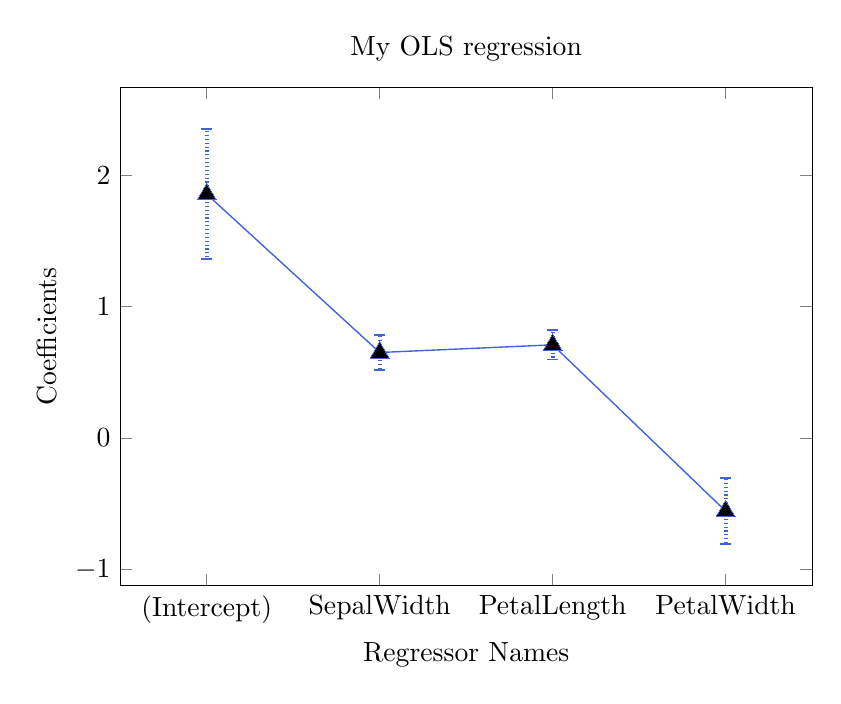
\begin{tikzpicture}
\begin{axis}[title={My OLS regression}, title style={}, xlabel={Regressor Names}, xlabel style={}, ylabel={Coefficients}, ylabel style={}, xticklabel style={}, yticklabel style={}, width={250pt}, height={180pt}, symbolic x coords={{(}Intercept{)},SepalWidth,PetalLength,PetalWidth}, xtick={{(}Intercept{)},SepalWidth,PetalLength,PetalWidth}, xmin={{[normalized]-0.5}}, xmax={{[normalized]3.5}}, scale only axis]
    \addplot[mark={triangle*}, mark options={mark size={4pt}, line width={0pt}}, error bars/error mark={|}, error bars/error mark options={mark size={2.0pt}, solid, line width={0.6pt}, fill={rgb,255: red, 64; green, 99; blue, 216}, fill opacity={1}, draw={rgb,255: red, 64; green, 99; blue, 216}, draw opacity={1}}, error bars/error bar style={draw={rgb,255: red, 64; green, 99; blue, 216}, draw opacity={1}, densely dotted, line width={1.5pt}}, draw={rgb,255: red, 64; green, 99; blue, 216}, draw opacity={1}, line width={0.5pt}, error bars/y dir={both}, error bars/y explicit]
        coordinates {
            ({(}Intercept{)},1.8559974929173773) +- (0,0.49562225706653434)
            (SepalWidth,0.6508371593132527) +- (0,0.13171828828576346)
            (PetalLength,0.7091319591367713) +- (0,0.11209691841093013)
            (PetalWidth,-0.5564826601671072) +- (0,0.2520788358782843)
        }
        ;
\end{axis}
\end{tikzpicture}
\end{document}
